\section{Plugin Architecture} \label{subsec_plugin_architecture}

The Expander Framework artifact is responsible for loading and bootstrapping Expanders and
initiating the generation process. Expanders are dynamically loaded at runtime through a
dotnet capability called assembly binding, allowing the architecture illustrated in the
following image \parencite{koks_expanderpluginloaderinteractor_2023}.

\begin{figure}[H]
  \centering
  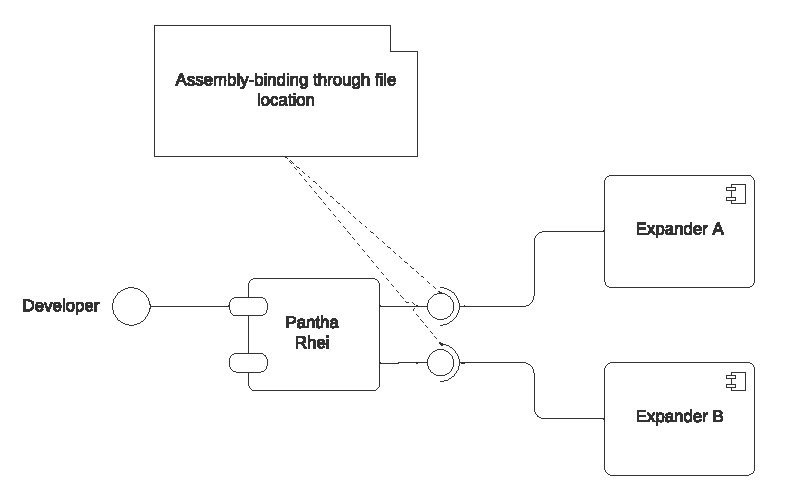
\includegraphics[width=0.5\textwidth]{figures/plugin_architecture.pdf}
  \caption[Plugin Archticture]{Expanders are considered plugins}
  \label{fi:plugin_architecture}
\end{figure}

This plugin design adheres to several principles of \gls{solid}. The \gls{srp} principle
is implemented by ensuring that an expander generates one and only one construct. The
\gls{ocp} principle is applied by allowing the creation of new expanders in addition to
the already existing ones. The \gls{lsp} principle is respected by enabling the addition
or replacement of expanders without modifying the internal workings of the Expander
Framework.

More details can be found in Appendix \fullref{list_expanderpluginloaderinteractor}